\documentclass{article}

\usepackage[final, nonatbib]{neurips_2024}
\usepackage[numbers,compress]{natbib}
\usepackage[T1]{fontenc}
\usepackage[utf8]{inputenc}
\usepackage{amsmath,amssymb}
\usepackage{graphicx}
\usepackage{booktabs}
\usepackage{microtype}
\usepackage{hyperref}
\hypersetup{hidelinks}

\title{Clean Accuracy Is the Wrong Lens:\\
       Reading Invariance and Capacity from Digit Networks}

\author{%
  Attila Torda \\
  Independent Researcher \\
}

\begin{document}
\maketitle

\begin{abstract}
On MNIST, modern networks are separated by a fraction of a percentage point of test accuracy,
which invites the conclusion that the architecture no longer matters. We argue the opposite: clean
accuracy \emph{hides} what each network computes and needs, and two cheap readouts---perturbation
robustness and per-layer linear separability---recover it. (i)~A panel spanning an MLP, a small
CNN, and the MNIST record-holder model differs by only $1.4$ percentage points on clean data but by
$\sim\!46$~pp under a $4$-pixel shift: the architectural gap is an \emph{invariance} gap, invisible
on clean accuracy and ordered exactly by spatial structure. (ii)~A depth ablation shows clean
accuracy and per-layer linear separability both saturate at $\sim\!4$ convolutional blocks---beyond
which the representation is already linearly separable, so no non-linearly-separable
(``XOR-like'') classification work remains---yet translation robustness keeps improving with depth,
giving a concrete capacity rule: few layers suffice for clean accuracy, more buy invariance.
(iii)~The networks also carry recoverable latent structure: an unsupervised style variant
(crossed vs.\ uncrossed ``7'') is linearly decodable \emph{and} generatively steerable, and depth
makes internal class prototypes clean. The unifying message is that robustness and linear
separability, not clean accuracy, are the informative axes for reading digit networks.
\end{abstract}

\section{Introduction}
MNIST \cite{LeCun1998} is often treated as solved: the reproducible record is $99.87\%$
\cite{An2020} and competing architectures cluster within a percentage point. This near-saturation
makes clean test accuracy almost useless for \emph{comparing} or \emph{understanding} digit
networks. We show that two inexpensive measurements recover the information that clean accuracy
hides, and that they tell a consistent story.

Our contributions are three readouts and one unifying claim. \textbf{(1) Model differences are
invariance differences}, readable from perturbation robustness rather than clean accuracy.
\textbf{(2) Depth past a linear-separability ``knee'' buys robustness, not accuracy}---a concrete,
actionable capacity rule obtained from a depth ablation plus per-layer linear probes
\cite{Alain2017}. \textbf{(3) Digit networks carry recoverable latent structure}: an unsupervised
style variant is both linearly decodable and generatively steerable, and depth yields clean
internal class prototypes (via activation maximization \cite{Erhan2009,Simonyan2014,Olah2017}).
The unifying claim: \emph{robustness and linear separability are the informative axes; clean
accuracy is the wrong lens.}

\section{Setup}
All models are trained on MNIST with one backbone family per experiment. The comparison panel is
an \textbf{MLP} ($784\!-\!256\!-\!128\!-\!10$), the $2$-conv \textbf{SimpleCNN}, and \textbf{M3},
the single deepest sub-model ($10$ conv layers, no pooling) of the An et al.\ record holder
\cite{An2020}. The depth study uses a \textbf{DepthCNN} family of $1$--$8$ identical conv blocks.
We perturb the test set by integer translation and rotation (\texttt{torchvision} affine), fit
linear probes (logistic regression) on intermediate features, and reconstruct ``canonical''
class images by gradient ascent on the input with total-variation/blur regularization. All numbers
are means over $3$ seeds.

\section{Reading 1: model differences encode invariance}
Table~\ref{tab:panel} and Figure~\ref{fig:robust} report the panel. On clean MNIST the three
architectures span just $1.4$~pp ($98.08 / 99.12 / 99.47$)---they look nearly equivalent. Under a
$4$-pixel shift they span $\sim\!46$~pp ($39.7 / 71.7 / 85.8$): the MLP, with no spatial prior,
collapses; the convolutional prior recovers much of it; and depth without pooling (M3) recovers
most. The ordering MLP $\ll$ SimpleCNN $\ll$ M3 is identical for translation and rotation. Thus
``model $A$ beats model $B$'' is best read as ``$A$ computes more invariance,'' a statement clean
accuracy cannot make. \textbf{Honest null:} an unsupervised style-variant probe (\S\ref{sec:latent})
reaches $\sim\!80\%$ on \emph{all three} representations (base $57\%$)---structure preservation is
architecture-independent, so the discriminating axis is robustness, not representation richness.

\begin{table}[t]
\caption{Panel (3 seeds): clean accuracy barely separates the models; robustness does.}
\label{tab:panel}
\centering
\begin{tabular}{@{}lcccc@{}}
\toprule
Model & Clean acc & Acc @ 4px shift & Acc @ 20$^\circ$ rot & variant-7 probe (base 57) \\
\midrule
MLP        & 98.08 & 39.7 & 87.1 & 80.1 \\
SimpleCNN  & 99.12 & 71.7 & 93.4 & 79.2 \\
M3 (record) & \textbf{99.47} & \textbf{85.8} & \textbf{95.3} & 79.9 \\
\bottomrule
\end{tabular}
\end{table}

\section{Reading 2: depth past the linear-separability knee buys robustness, not accuracy}
\label{sec:depth}
A classic fact motivates the question: a single linear unit cannot compute XOR, the smallest
non-linearly-separable function \cite{Minsky1969}; depth exists to implement such functions. So if
a network's representation is already \emph{linearly} separable for the task at layer $L$, layers
beyond $L$ do no further non-linearly-separable (``XOR-like'') classification work, and one might
cut them. We test this directly (Figure~\ref{fig:depth}). Training DepthCNNs of $1$--$8$ blocks,
clean accuracy saturates by $\sim\!4$ blocks ($99.06\to99.27$ from block $3$ to $8$). A per-layer
linear probe on the $8$-block net confirms the cause: a \emph{linear} classifier already reaches
$99.1\%$ by block $4$ (final $99.5\%$), i.e.\ the representation is linearly separable there.
\emph{However}, translation robustness keeps climbing well past the knee: acc@4px $=91.5$ (d3)
$\to95.5$ (d4) $\to98.5$ (d8). The resulting \textbf{capacity rule}: for clean MNIST accuracy
$\sim\!4$ blocks suffice and deeper is wasted; if invariance/robustness matters, extra depth keeps
paying. This is the same axis as Reading~1---added capacity buys robustness, not clean accuracy.

\begin{figure}[t]
\centering
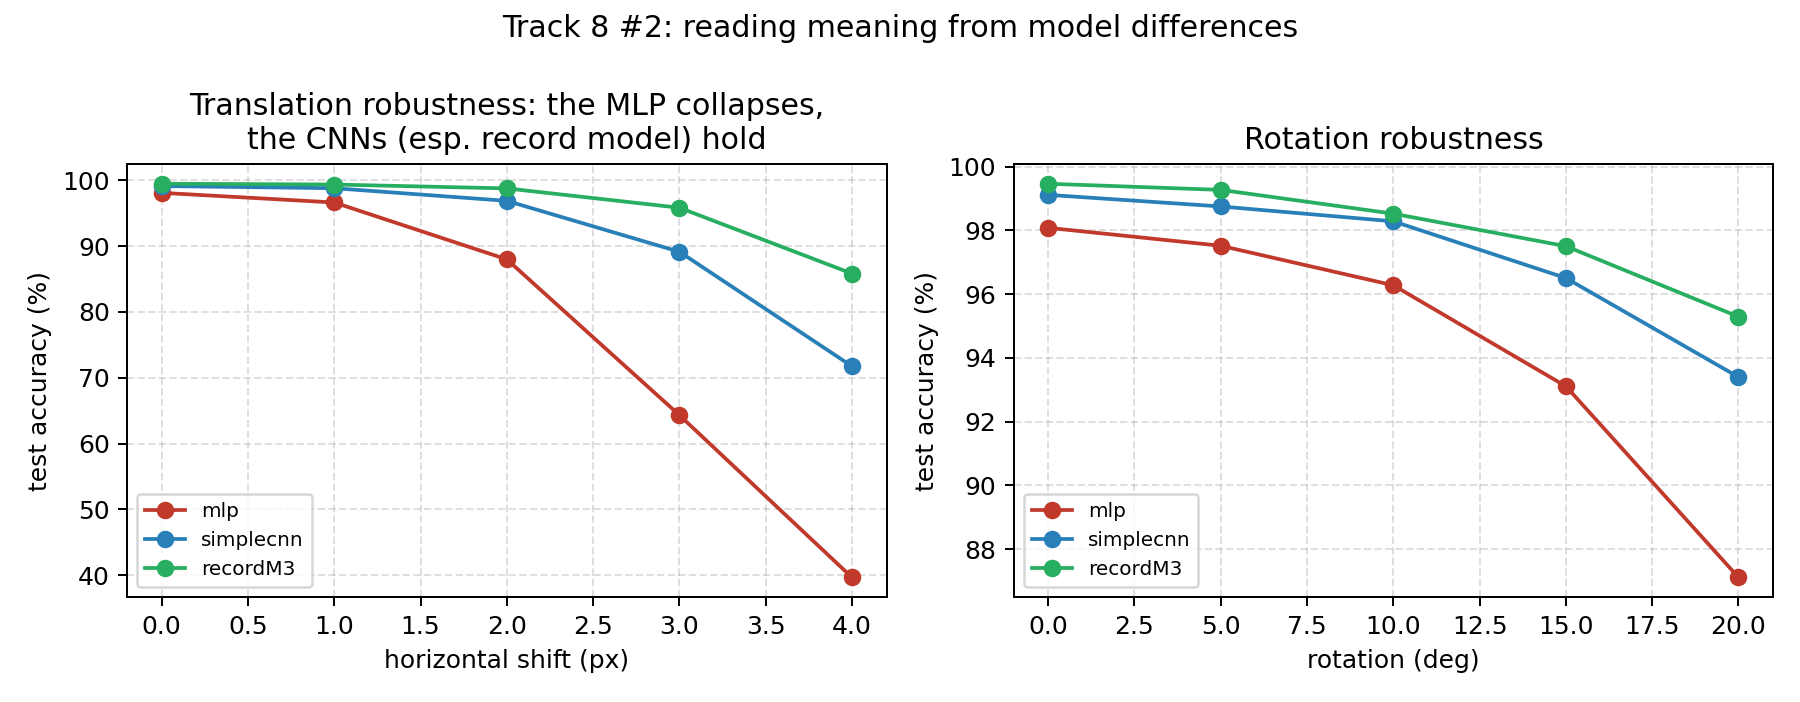
\includegraphics[width=0.92\linewidth]{figures/fig_track8_panel_robust.png}
\caption{Reading~1. Clean ($0$ shift) the three models coincide at $\sim\!98$--$99\%$; under
perturbation they fan out by tens of points, ordered by spatial structure. The architectural
difference is an invariance gap.}
\label{fig:robust}
\end{figure}

\begin{figure}[t]
\centering
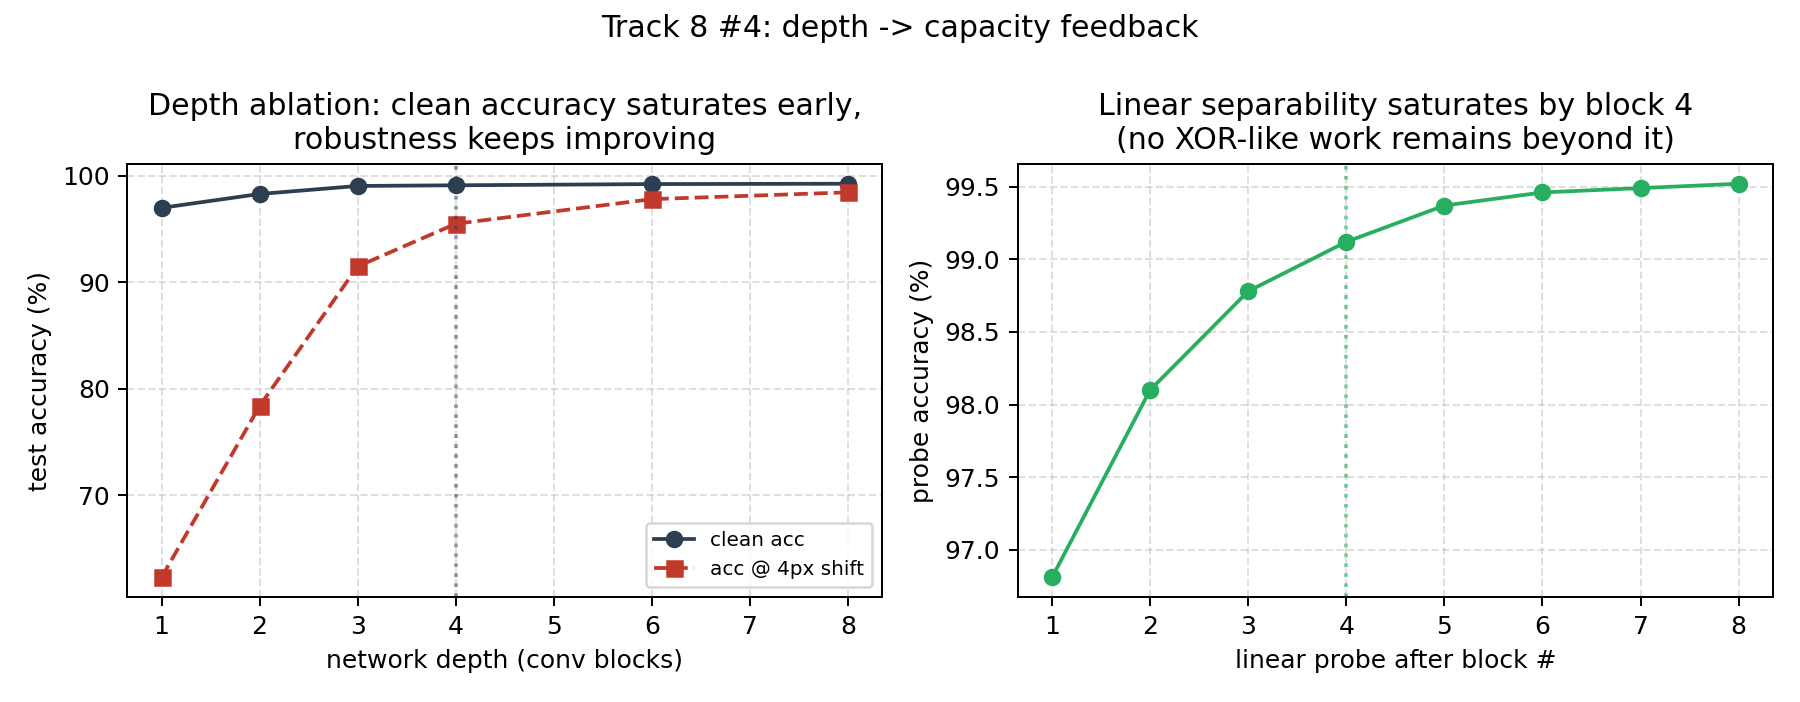
\includegraphics[width=0.92\linewidth]{figures/fig_track8_depth.png}
\caption{Reading~2. Left: clean accuracy saturates by $\sim\!4$ blocks while $4$-px-shift
robustness keeps rising with depth. Right: a per-layer linear probe saturates by block $4$---no
``XOR-like'' work remains beyond it, so the leftover gains from depth are invariance, not
separability.}
\label{fig:depth}
\end{figure}

\section{Reading 3: recoverable latent structure and clean prototypes}
\label{sec:latent}
\textbf{Decodable + generative style variant.} A plain $10$-class CNN never sees style labels, yet
a crossed-vs-uncrossed ``7'' variant (defined from the skeleton graph \cite{GuoHall1989}) is
linearly decodable from its embedding ($83.8\%$ probe vs.\ $57\%$ base). The axis is not merely
decodable but \emph{generative}: reconstructing a ``7'' while pushing its embedding along the probe
direction moves the variant score monotonically ($-8.2\to+25.0$) and adds/removes crossbar
structure---so the network can be driven to render either variant.

\textbf{Depth yields clean prototypes.} Activation-maximizing each class
(Figure~\ref{fig:proto}) shows the deep record sub-models render smooth, prototype-like canonical
digits (mean total variation $\sim\!0.08$) where the shallow SimpleCNN renders high-frequency
texture that barely resembles a digit (TV $\sim\!0.5$). Smoothness tracks \emph{depth}, not kernel
size; the three record sub-models' templates differ, consistent with their ensemble's decorrelation.

\begin{figure}[t]
\centering
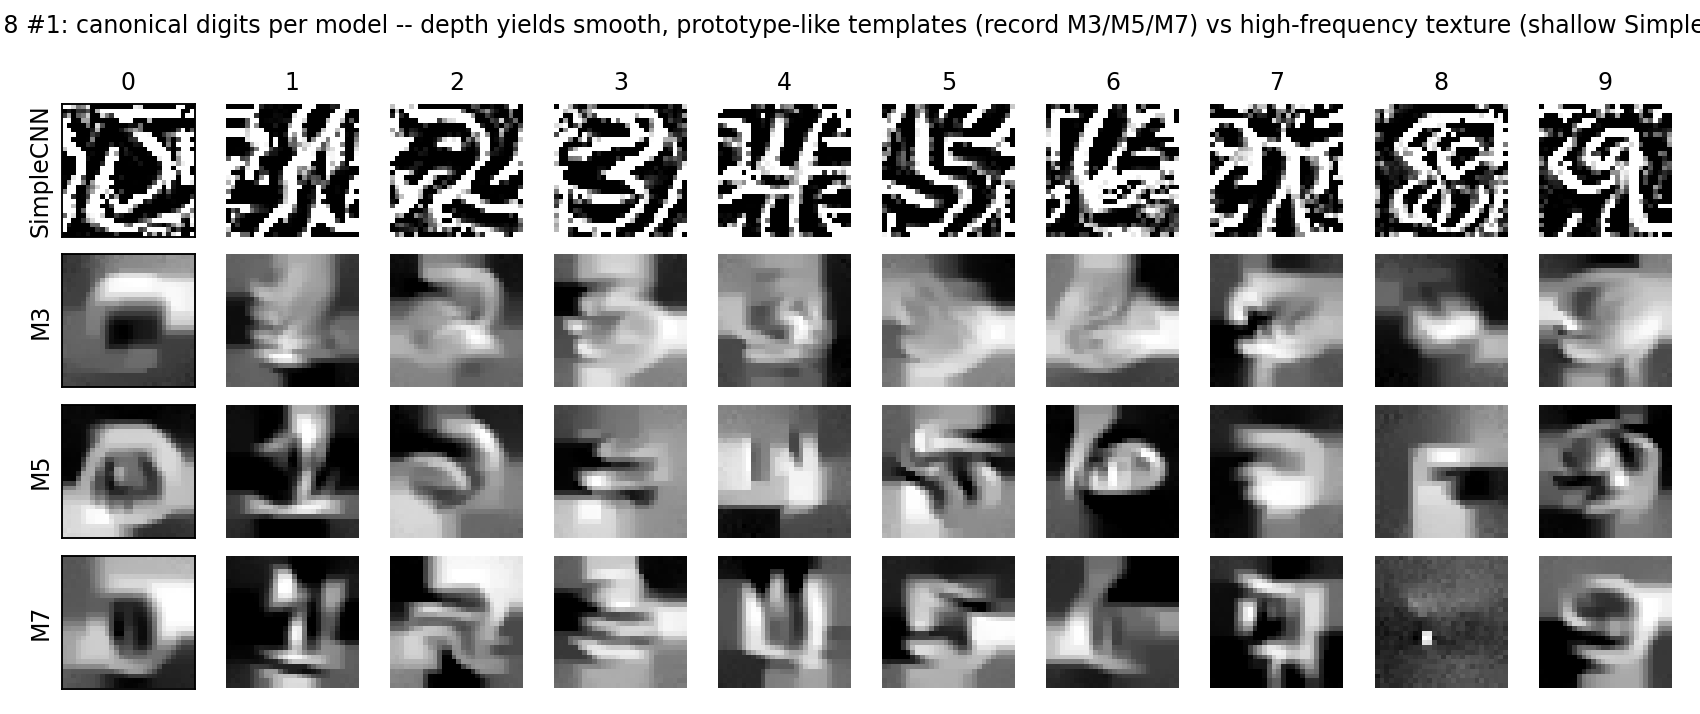
\includegraphics[width=0.92\linewidth]{figures/fig_track8_receptive_fields.png}
\caption{Reading~3. ``Canonical'' class images by activation maximization. The deep record
sub-models (M3/M5/M7) form smooth, prototype-like digits; the shallow CNN forms high-frequency
texture.}
\label{fig:proto}
\end{figure}

\section{Discussion}
The three readings agree on one axis. Clean accuracy is saturated and near-constant across
architectures and depths; the variation that \emph{does} carry architectural meaning---which model
generalizes under shift, whether extra depth helps, what the network has internalized---shows up in
robustness and in linear separability, not in the headline number. Practically: compare models by
perturbation robustness, not clean accuracy; choose depth by the linear-separability knee unless
robustness is the goal; and remember that a discriminative digit net carries decodable, steerable
generative structure.

\textbf{Limitations.} This is MNIST and a small model family; the individual tools (activation
maximization, linear probes, robustness evaluation) are established---our contribution is the
\emph{synthesis} and the concrete digit-network reading, not new machinery. The capacity rule is a
demonstrated trend on this task, not a theorem, and ``no XOR-like work remains'' is an operational
statement about linear-probe saturation, not a circuit-level claim.

\section{Conclusion}
On a near-saturated benchmark, clean accuracy is the wrong lens. Perturbation robustness reveals
that model differences are invariance differences; per-layer linear separability reveals that depth
past a knee buys robustness rather than accuracy; and activation maximization plus linear probes
reveal recoverable, steerable latent structure. Read digit networks by what they are robust to and
by where they become linearly separable---not by the last decimal of test accuracy.

\begin{ack}
Reproducibility: \texttt{scripts/run\_track8\_model\_panel.py} (Reading 1),
\texttt{run\_track8\_depth.py} (Reading 2), \texttt{run\_track8\_introspect\_best.py} +
\texttt{run\_introspection\_reconstruct.py} (Reading 3). Raw results:
\texttt{track8\_panel\_results.json}, \texttt{track8\_depth\_results.json}; full notes in
\texttt{cnn\_introspection\_findings.md}.
\end{ack}

\bibliographystyle{plainnat}
\bibliography{track8_refs}

\end{document}
